%% Springer Nature LaTeX template (sn-jnl) — Scientific Reports submission.
%% Compiles with pdflatex (two passes for cross-references/citations).
\documentclass[lineno,pdflatex,sn-basic,Numbered]{sn-jnl}

\usepackage{graphicx}
\usepackage{multirow}
\usepackage{amsmath,amssymb,amsfonts}
\usepackage{booktabs}
\usepackage[T1]{fontenc}

\raggedbottom

\begin{document}

\title[Foundation-model choice and false-positive burden in LLM AML screening]{The choice of foundation model determines the false-positive burden of large language model anti-money-laundering transaction screening}

\author[1]{\fnm{Samir} \sur{Chincholikar}}\email{samir.chincholikar@gmail.com}

\author*[1]{\fnm{Robin} \sur{Chawla}}\email{robin.chawla.cse14@iitbhu.ac.in}

\affil*[1]{\orgname{Independent Researcher}}

\abstract{Large language models are being adopted to screen financial transactions for money laundering, but the consequences of choosing one foundation model over another have not been measured. We evaluated five widely used foundation models as zero-shot anti-money-laundering screeners on an identical, preregistered set of 600 synthetic cases anchored to recognised laundering typologies, half of them legitimate transactions designed to resemble alerts. On the same legitimate transactions, the rate at which models raised a false alarm ranged from 0.3\% to 83.0\%, a difference of 83 percentage points, and the models disagreed on 86\% of legitimate cases. The variation was systematic: within each provider the false-alarm rate fell monotonically as model capability rose, so the smallest, cheapest models over-flagged (83.0\%) while their flagship siblings did not (1.0\%). Each model therefore occupies a different point on the trade-off between catching laundering and over-flagging legitimate activity, and because institutions commonly substitute a cheaper model to cut cost, that choice moves a deployment toward a high-false-positive regime. Projected to realistic conditions, this choice changes the daily alert workload about two hundred--fold. Because the model behind a commercial interface can change without notice, this operating point is an unmanaged risk that current oversight does not capture.}

\keywords{anti-money laundering, large language models, false positives, model risk, transaction monitoring, foundation models}

\maketitle

\section{Introduction}\label{sec:intro}

Money laundering is estimated to move the equivalent of 2--5\% of global gross domestic product each year, and financial institutions are legally obliged to monitor transactions and to report suspicious activity to the authorities \cite{fatf-tbml,unodc}. The dominant technology for this task---rules-based transaction monitoring---is widely criticised for generating enormous volumes of false alarms, commonly cited as exceeding 90\% of all alerts, which impose heavy analyst review costs and drive the ``de-risking'' of legitimate customers and correspondent banks \cite{srguidance}. This false-positive burden, rather than raw detection accuracy, is the central operational problem of anti-money-laundering (AML) compliance, and it is the problem that machine-learning approaches to transaction monitoring have primarily sought to reduce, typically by addressing the severe class imbalance of the data \cite{smote,imbalance,srfraud1,srfraud2}.

Large language models (LLMs)---general-purpose foundation models trained on broad data and adapted to many tasks through natural-language instructions \cite{fewshot,foundation}---are now being proposed and piloted as flexible AML screeners. Unlike a bespoke classifier, an instruction-followed LLM can read heterogeneous transaction context and reason about laundering typologies without task-specific training, which is attractive to institutions seeking to modernise legacy monitoring. A rapidly growing literature evaluates LLMs and other machine-learning methods for financial-crime detection, spanning credit-card fraud, healthcare-claims fraud, temporal-drift robustness and federated learning \cite{srfraud1,srfraud2,srfraud3,srfraud4}. Almost all of this work is framed around a capability question: how accurately can a given model detect fraud or laundering. That framing implicitly treats ``an LLM'' as a single, interchangeable component, and it evaluates one model, or compares models only to identify the most accurate one---mirroring the model-centric emphasis of general LLM evaluation and of the broader debate over the reliability of large models \cite{helm,parrots}.

Two features of that literature are worth making explicit, because our results speak to both. First, the defining statistical challenge in financial-crime detection is extreme class imbalance: genuinely suspicious activity is rare, so a large body of work concentrates on resampling and cost-sensitive learning---most prominently the synthetic minority over-sampling technique and its many hybrids---and on comparing dozens of classical, ensemble and deep models to minimise the false-positive rate at a fixed recall \cite{smote,imbalance,srfraud1,srfraud2}. Recent studies extend this toolkit with generative and federated architectures and with post-hoc explainability such as SHAP and LIME \cite{shap,lime} to make individual alerts auditable, and with drift-aware frameworks that monitor a deployed model for degradation as transaction patterns evolve over time \cite{srfraud3,srfraud4}. Second, and central to our argument, all of this work shares an implicit assumption: that the model, once selected, trained or validated, is a fixed artefact whose behaviour changes only through retraining or measurable concept drift. A bespoke classifier trained in-house satisfies that assumption. A foundation model accessed through a commercial interface does not: its weights are controlled by the provider, are opaque to the institution, and can be replaced, re-priced or retired without notice and without any retraining event that a drift monitor would observe. The false-positive problem that the fraud-detection literature seeks to reduce through better models and resampling is, we show, also created---across two orders of magnitude---simply by which foundation model is placed behind the screener, before any tuning has taken place; and the explainability tools that make a single alert auditable do not surface the fact that an equally plausible alternative model would have produced a different alert at a different rate. These observations motivate treating foundation-model selection itself, rather than only model accuracy, as an object of measurement and governance.

We therefore ask a different question, and argue that for governance it is the more consequential one: holding the screening task fixed, how much does the choice of foundation model change the outcome? Institutions that access LLMs through commercial application programming interfaces (APIs) choose among several providers and among several model versions of differing size and price, and providers routinely update, re-price and retire those versions. If two otherwise-identical deployments that screen the same activity with two different models produce materially different false-alarm rates, then a decision currently treated as procurement---which model to call---silently sets a core risk parameter. This concern is sharpened by a parallel line of work on ``algorithmic monoculture,'' which warns that when many institutions build on the same foundation models their decisions may homogenise and their errors correlate, creating systemic fragility and a form of arbitrariness in who is subjected to a given automated judgment \cite{monoculture,homogenization,leviathan}. Whether shared foundation models in AML screening produce homogenisation, divergence, or neither has not, to our knowledge, been measured.

Here we provide that measurement. Using a preregistered, fully reproducible design, we ran five foundation models from two providers as zero-shot screeners over an identical battery of 600 synthetic cases anchored to the Financial Action Task Force (FATF) typology catalogue and to established synthetic-AML data structures \cite{samld,amlsim}. On identical legitimate transactions, per-model false-positive rates spanned two orders of magnitude; within each provider the rate fell monotonically as model capability rose, so that cheaper, smaller models over-flagged far more; and each model implied a different operating point on the sensitivity--specificity trade-off. We quantify the operational consequence for alert volume, locate the models against rules-based and supervised baselines, and argue that the operating point of an LLM screener---and its instability under provider-driven model substitution---must be brought inside model-risk governance. We also report, as a preregistered secondary analysis, that the models did \emph{not} exhibit correlated misses: rather than homogenising, their false alarms diverged sharply and idiosyncratically.

\section{Results}\label{sec:results}

\subsection{Foundation models diverge by 83 percentage points in false-positive rate on identical transactions}\label{sec:fpspread}

Each of five models---GPT-4o-mini, GPT-4.1-mini and GPT-4o (OpenAI), and Gemini Flash and Gemini Flash-Lite (Google)---screened all 600 cases under two prompt phrasings and two random seeds, returning a structured suspicious/not-suspicious decision (Methods). A false positive is a legitimate (``benign'') case flagged as suspicious; a miss is a suspicious case not flagged. Per-case decisions were the majority vote over the four replicates.

On the 300 legitimate cases, false-positive rates ranged from 0.3\% (Gemini Flash; 1 of 300) to 83.0\% (GPT-4o-mini; 249 of 300)---a spread of 82.7 percentage points (95\% confidence interval [CI] 69.2--95.3, cluster bootstrap over typology strata) (Fig.~\ref{fig:fp}, Table~\ref{tab:ops}). The five models differed in false-positive rate far beyond chance (Cochran's $Q = 131.6$, degrees of freedom $= 4$, $P \approx 2\times10^{-27}$; the five models are related raters scored on the same cases). They fell into three statistically distinct tiers: pairwise McNemar exact tests (Bonferroni-corrected across the ten model pairs, two-tailed) separated the two cautious models (Gemini Flash, GPT-4o) from the two intermediate models (GPT-4.1-mini, Gemini Flash-Lite) from GPT-4o-mini, with every between-tier comparison at $P < 10^{-19}$, while the two within-tier comparisons were not distinguishable ($P = 1.0$) (Table~\ref{tab:mcnemar}). Across models, the flag decision was not unanimous on 85.7\% of legitimate cases (95\% CI 75.1--95.4).

\subsection{False-positive rate falls monotonically with model capability within each provider}\label{sec:nonmono}

The variation is not idiosyncratic but highly systematic: within each provider, the false-positive rate decreases monotonically as model capability (and price) increases (Fig.~\ref{fig:ops}, Table~\ref{tab:ops}). In the OpenAI family, the smallest model GPT-4o-mini flagged 83.0\% of legitimate cases, the intermediate GPT-4.1-mini 23.7\%, and the flagship GPT-4o only 1.0\%; in the Google family, the smaller Gemini Flash-Lite flagged 24.7\% and the more capable Gemini Flash only 0.3\%. In both families, without exception, the cheaper, smaller model is the more over-flagging one.

This monotonic dependence does not weaken the governance concern---it sharpens it. Because a model's price tracks its capability, the most common cost optimisation in production LLM deployments---routing traffic from a flagship model to a smaller, cheaper variant---moves a deployment predictably and steeply toward a high-false-positive operating point, and providers can perform such substitutions silently. The risk is therefore not that model choice has unpredictable effects, but that the default choice under cost pressure (the cheapest model) is systematically the worst on false positives, while the trade-off is undisclosed and ungoverned. Capability does not, however, rescue LLM screening: the flagships' low false-positive rates are bought at a recall cost (Gemini Flash missed 12.0\% of suspicious cases; Table~\ref{tab:ops}), the cheap models' near-perfect recall is bought at catastrophic false-positive rates, and a tuned classifier and even a rules baseline dominate the cheaper models (Fig.~\ref{fig:ops}). Finally, the cross-model dispersion is concentrated at the low-capability tier: the two smallest models differ by 58 percentage points (24.7\% vs 83.0\%), whereas the two flagships converge near zero (0.3\% vs 1.0\%)---so provider choice matters most precisely where cost pressure pushes institutions.

Plotting each model by its false-positive rate and its sensitivity (the fraction of suspicious cases caught) shows the models scattered across the operating curve (Fig.~\ref{fig:ops}): GPT-4o-mini sits at maximum sensitivity and minimum specificity (it catches essentially everything, but flags 83\% of legitimate activity), whereas Gemini Flash is highly specific but misses 12.0\% of suspicious cases. The choice of model therefore selects an entire operating point---a miss-prone regime or an alert-flooding regime---not merely a level of ``accuracy.''

\subsection{The operating point translates into a two-hundred-fold difference in alert workload}\label{sec:volume}

Screening performance on a balanced battery measures discrimination; operational burden depends on the low real-world prevalence of suspicious activity and is dominated by false positives. Projecting each operating point to a representative institution processing 1,000,000 transactions per day at a suspicious prevalence of 0.1\% (Fig.~\ref{fig:vol}, Table~\ref{tab:vol}), the daily alert queue ranges from about 4,200 alerts (Gemini Flash) to about 830,000 (GPT-4o-mini)---a roughly 197-fold difference on identical activity---while the fraction of alerts that are genuinely suspicious (precision) collapses from 20.9\% to 0.12\%. At the GPT-4o-mini operating point, approximately 999 of every 1,000 alerts are false.

\subsection{Locating the models against non-LLM baselines}\label{sec:baselines}

To provide a reference frame we evaluated two non-LLM screeners on the identical 600 cases (Methods). A deterministic rules baseline encoding FATF red-flag heuristics produced a 12.0\% false-positive rate with an 11.3\% miss rate, and a supervised classifier (gradient boosting on engineered features, evaluated out-of-fold) achieved near-zero false positives and misses. The task is therefore not intrinsically difficult: a tuned classifier separates the classes almost perfectly, and even a simple rules system reaches a 12\% false-positive rate. Against this frame (Fig.~\ref{fig:ops}, Table~\ref{tab:vol}), the LLMs are dispersed across---and frequently worse than---the incumbent baselines: GPT-4o-mini's false-positive rate is roughly seven times that of the rules baseline, whereas GPT-4o and Gemini Flash are competitive with a tuned classifier on false positives. The dispersion is thus a property of using untuned foundation models, whose operating points are inherited rather than chosen.

\subsection{A shared trade-based blind spot, prompt sensitivity that preserves the ordering, and no correlated misses}\label{sec:typology}

Where the models do miss, they miss together on specific typologies (Fig.~\ref{fig:typ}). Pooled across models, trade-based laundering was missed 18.9\% of the time (95\% CI 14.0--25.1) and cash-intensive fronts 10.3\%, whereas structuring, layering, mule networks, funnel accounts, shell layering and rapid pass-through were caught almost perfectly (miss rates $\leq 1.6\%$). The miss pattern is itself heterogeneous across models (Fig.~\ref{fig:heat}): the cautious models that rarely false-alarm (Gemini Flash, GPT-4o) account for most of the trade-based and cash-intensive misses, whereas the alert-flooding GPT-4o-mini misses almost nothing---a per-typology view of the same operating-point trade-off. Trade-based laundering, which turns on economic-substance judgements not visible in transaction structure, is thus the typology where human escalation remains necessary regardless of model choice. Prompt phrasing shifted each model's operating point in a consistent direction---the FATF-typology prompt was uniformly the more aggressive, raising every model's false-positive rate (Gemini Flash 0.3\%$\rightarrow$2.3\%, GPT-4o 0.3\%$\rightarrow$7.7\%, GPT-4.1-mini 20.7\%$\rightarrow$36.7\%, Gemini Flash-Lite 24.7\%$\rightarrow$44.0\%, GPT-4o-mini 78.7\%$\rightarrow$85.0\%). This within-model shift (2--19 percentage points; overall decision-flip rate 7.5\%, 95\% CI 6.9--8.2) was small relative to the between-model divergence and preserved the tier ordering, so the divergence is a property of the models rather than an artefact of a particular prompt \cite{promptsens}. Finally, as a preregistered secondary analysis we tested the competing algorithmic-monoculture prediction that shared foundation models would fail on the \emph{same} cases. We found the opposite: no suspicious case was missed by all five models, per-model miss rates were low (0.0--12.0\%), and chance-corrected agreement on the miss label was near zero (mean pairwise Cohen's $\kappa = 0.072$; range $-0.011$ to $0.26$; consistent under Scott's $\pi$ and Gwet's AC1, Supplementary Information). The robust cross-model effect is therefore divergence in false alarms, not homogenisation of misses.

\section{Discussion}\label{sec:discussion}

On identical transactions, the choice of foundation model swings the AML false-alarm rate across two orders of magnitude, this variation falls monotonically with model capability within each provider so that cheaper, smaller models over-flag far more, and it translates into a roughly two-hundred-fold difference in analyst workload at realistic prevalence. The operating point that governs an institution's suspicious-activity workload, its rate of de-risking legitimate customers, and its residual exposure to missed laundering is therefore set by a model-selection decision that is currently treated as procurement rather than as a governed risk parameter. This is not the claim that institutions will knowingly deploy a screener that false-alarms on 83\% of legitimate activity; a competent validation would detect that immediately. It is the claim that the operating point is undisclosed by providers, that it tracks the model's capability and hence its price---so that cost-driven substitution moves it predictably toward more false alarms---and that it can move without any action by the institution. A provider that upgrades a model, re-routes traffic from a flagship to a cheaper variant to reduce cost, or retires a version can move a deployment from one column of Table~\ref{tab:ops} to another---potentially a hundred-fold change in alert burden---with no model-inventory event and no revalidation trigger. We encountered this instability directly: during data collection a provider deprecated the model snapshots we had selected, forcing a substitution to a differently behaving model. Supervisory guidance on model risk management already requires that vendor and third-party models be inventoried, validated and monitored under consistent principles \cite{srguidance}, and emerging AI-governance frameworks and regulation extend comparable expectations to AI systems used in high-stakes settings \cite{nistrmf,aiact}; our results identify a specific, measurable and currently ungoverned risk channel within that mandate---the operating point implied by model selection and its drift under substitution. Three practices follow: treat the model snapshot, not merely ``the provider's API,'' as the inventoried model, so that a substitution is a governance event; require disclosure or measurement of the false-positive and miss operating point on a standard battery before and after any model change, in the spirit of standardised model and dataset documentation \cite{modelcards,datasheets}; and back-test heterogeneously and audit end-to-end \cite{accountability}, because a single accuracy number conceals the operating-point divergence documented here. These practices target a gap that existing model-risk tooling does not close. Drift monitors watch a fixed model for degradation as data evolve, but a provider-side model substitution is not data drift and produces no gradual signal for them to detect; post-hoc explainability makes an individual alert auditable but is silent on the counterfactual that a different, equally defensible model would have raised a different alert at a different rate; and champion--challenger validation compares candidate models at selection time but is rarely re-run when a vendor silently swaps the model beneath a live interface. A practical, low-cost control that follows directly from our design is a standing ``operating-point probe'': a fixed, held-out battery of labelled benign and suspicious cases, screened automatically on a schedule and on every model-version change, with the measured false-positive and miss rates logged to the model inventory and alerted on when they move beyond a tolerance. The alert-volume projection (Table~\ref{tab:vol}) offers a template for expressing that operating point in the currency supervisors and operations teams use---expected alert queue and precision at the institution's own prevalence---so that a change in the model behind the interface becomes a visible, governed event rather than an invisible shift in analyst workload and de-risking exposure. Our results also bear on the algorithmic-monoculture hypothesis: we preregistered and tested whether shared foundation models would miss the same cases, and found the opposite for false alarms---sharp, idiosyncratic divergence rather than homogenisation---which calls for disclosure and operating-point control rather than enforced heterogeneity. Several limitations bound these conclusions. The battery is synthetic by necessity rather than convenience: real transaction records carrying ground-truth laundering labels cannot be shared, because suspicious-activity determinations are confidential by statute and customer transactions are protected by financial-privacy and data-protection law, so typology-anchored synthetic batteries (SAML-D, AMLSim) are the standard evaluation substrate in this field \cite{samld,amlsim}. Consequently, although the battery is anchored to FATF typologies and built with hard negatives, absolute rates will differ on production data, and we measure discrimination on a balanced set and project to operational prevalence rather than measuring against real alert dispositions. A second limitation concerns model identification: two of the five models (the Gemini pair) were reachable only through undated ``-latest'' aliases (Methods), so their exact snapshot cannot be pinned in the way the OpenAI models can---a constraint imposed by the provider that both weakens reproducibility for those two models and directly illustrates the disclosure gap this paper argues must be closed. The study covers five models from two providers, a snapshot of mid-2026, and does not include reasoning or open-weight models, so the monotone capability--false-positive relationship, although consistent across both families here, should be confirmed on additional providers, reasoning models and open-weight models. The supervised baseline is an optimistic ceiling on synthetic structure, and we evaluate zero-shot screeners, whereas a production deployment would tune and threshold---the governance gap we identify concerns precisely the substitution of the underlying model beneath such a deployment. Within these bounds, the finding is robust across two prompt phrasings, two seeds, chance-corrected agreement statistics and cluster-bootstrap resampling, and it is reproducible end-to-end from frozen data. The practical message for institutions and supervisors is that foundation-model selection in AML screening is a first-class model-risk decision: the model behind the interface, and any change to it, must be inventoried, its operating point disclosed and monitored, and human escalation preserved for economic-substance typologies such as trade-based laundering whichever model is chosen.

\section{Conclusion}\label{sec:conclusion}

We measured, on identical transactions, how much the choice of foundation model changes the outcome of large language model anti-money-laundering screening, and found that it changes it enormously: false-positive rates on legitimate activity ranged from 0.3\% to 83\% across five widely used models, this variation fell monotonically with model capability within each provider so that cheaper, smaller models over-flagged far more, and it projects to a roughly two-hundred-fold difference in analyst alert workload at realistic prevalence. Model choice thus silently selects an entire operating point on the sensitivity--specificity trade-off, and because the model behind a commercial interface can be upgraded, downgraded or retired without notice, that operating point is an unmanaged and drifting model risk rather than a fixed, validated property. The practical implication is narrow and actionable: foundation-model selection and substitution in AML screening should be treated as first-class model-risk events---the specific model snapshot inventoried, its false-positive and miss operating point disclosed, measured on a standard battery and monitored on every version change, and human escalation preserved for economic-substance typologies such as trade-based laundering. The preregistered design, frozen data and one-command reproducible capsule accompanying this work provide a template for such measurement.

\section{Methods}\label{sec:methods}

\textbf{Case battery.} We generated a deterministic, offline battery of 600 synthetic cases (seed 20260715) anchored to the FATF typology catalogue and to the structure of established synthetic-AML datasets (SAML-D; IBM AMLSim lineage) \cite{samld,amlsim}. Each case is a small transaction sub-network serialised as a plain-text ledger of accounts (with know-your-customer and jurisdiction attributes) and transfers (amount, date, direction, channel). Half the cases are suspicious, spanning eight typologies (structuring, layering, trade-based, mule networks, shell layering, funnel accounts, rapid pass-through, cash-intensive fronts); half are legitimate ``hard negatives''---patterns such as payroll, treasury sweeps, documented trade finance and marketplace payouts---constructed to superficially resemble alerting conditions so that a model flagging every case cannot score well. To avoid leaking the label, cases contain raw transaction logs only (no natural-language summary), use irregular sub-threshold amounts rather than uniform values, interleave the typology signal with legitimate background transactions, and disperse transactions in time. The battery generator, the resulting file and its SHA-256 hash are provided; the reproduction pipeline regenerates the battery from the seed and verifies the hash.

\textbf{Models and screening procedure.} Five foundation models were accessed through their providers' APIs at temperature 0: GPT-4o-mini (\texttt{gpt-4o-mini-2024-07-18}), GPT-4.1-mini (\texttt{gpt-4.1-mini-2025-04-14}) and GPT-4o (\texttt{gpt-4o-2024-11-20}) from OpenAI \cite{gpt4}, and Gemini Flash and Gemini Flash-Lite from Google \cite{gemini}, accessed via the provider's \texttt{gemini-flash-latest} and \texttt{gemini-flash-lite-latest} aliases, which at the capture date (July 2026) resolved to Gemini~3.5~Flash and Gemini~2.5~Flash-Lite respectively. We note that, unlike OpenAI's dated snapshot identifiers (e.g.\ \texttt{gpt-4o-mini-2024-07-18}), Google's public aliases did not expose an immutable, dated version string---itself a concrete instance of the disclosure gap our results motivate, and a limitation we return to below. Each model screened every case under two supervisory prompt phrasings (a concise compliance-officer instruction and an FATF-typology-aware instruction) and two random seeds, yielding $5\times2\times2\times600 = 12{,}000$ screening calls. Models returned a constrained JSON object indicating whether the activity was suspicious; unparsable or failed calls were recorded as errors (overall error rate 0.08\%) and excluded from the per-case majority vote. Provider models are updated and retired over time; one provider deprecated a selected snapshot during data collection, which we report as an instance of the substitution effect analysed here.

\textbf{Estimands and statistics.} The primary quantities are the per-model false-positive rate on the 300 legitimate cases and the spread (maximum $-$ minimum) across models; secondary quantities are cross-model disagreement on legitimate cases, per-typology miss rate, and prompt-variant decision change. Because the five models screen the same cases, they are related (paired) raters. We tested the overall difference in false-positive rate with Cochran's $Q$ test for $k$ related binary samples \cite{cochran} ($k=5$, $n=300$; degrees of freedom $=k-1=4$), and pairwise differences with McNemar's exact (binomial) test on discordant cases \cite{mcnemar}, two-tailed, $\alpha=0.05$, Bonferroni-corrected across the ten model pairs. Proportions are reported with 95\% Wilson score confidence intervals \cite{wilson}; the spread, divergence and per-typology rates additionally carry 95\% percentile confidence intervals from a cluster bootstrap \cite{bootstrap} that resamples the eight typology strata (2,000 resamples, seed 4242). We use ``significant'' only when accompanied by a $P$ value and otherwise use ``substantial'' or ``large.'' Chance-corrected agreement across models was additionally summarised with Cohen's $\kappa$, Scott's $\pi$ and Gwet's AC1 \cite{gwet} (Supplementary Information), where the correlated-miss null is also reported.

\textbf{Baselines.} On the identical 600 cases we evaluated (i)~a deterministic rules baseline encoding FATF red-flag heuristics (sub-threshold structuring, mule fan-in, shell-entity wires, high-risk-jurisdiction wires, rapid pass-through) and (ii)~a supervised baseline (logistic-regression and gradient-boosting classifiers on engineered graph features---counts of cash transfers, sub-threshold amounts, fan-in, shell entities, high-risk jurisdictions, temporal span), evaluated with 5-fold stratified out-of-fold prediction. Because the synthetic battery's structure encodes the typologies, the supervised baseline is an optimistic ceiling and is reported as such.

\textbf{Operational projection.} For an institution processing $N=1{,}000{,}000$ transactions per day at suspicious prevalence $p=0.001$, expected daily alerts are $\mathrm{FP}\cdot N(1-p) + (1-\mathrm{miss})\cdot Np$, false alerts $\mathrm{FP}\cdot N(1-p)$, and precision the ratio of true to total alerts; we report these per model and per baseline (Table~\ref{tab:vol}).

\textbf{Software and reproducibility.} Analyses used Python 3.12 with NumPy 2.2.6, scikit-learn 1.7.2 \cite{sklearn}, SciPy 1.15 and Matplotlib 3.10; data collection additionally used the OpenAI and Google Python SDKs. All analysis is deterministic and reproduces byte-identically from the frozen data. The complete code, frozen data, preregistration and a one-command reproducible capsule are available (see Data availability). No large language model is listed as an author; LLMs are the object of study, and any use of an LLM in drafting was limited to language editing under the authors' verification, consistent with the journal's authorship policy.

\textbf{Ethics.} This study used only synthetic data and did not involve human participants, human tissue or animals; no ethical approval was required.

\begin{figure}[t]
\centering
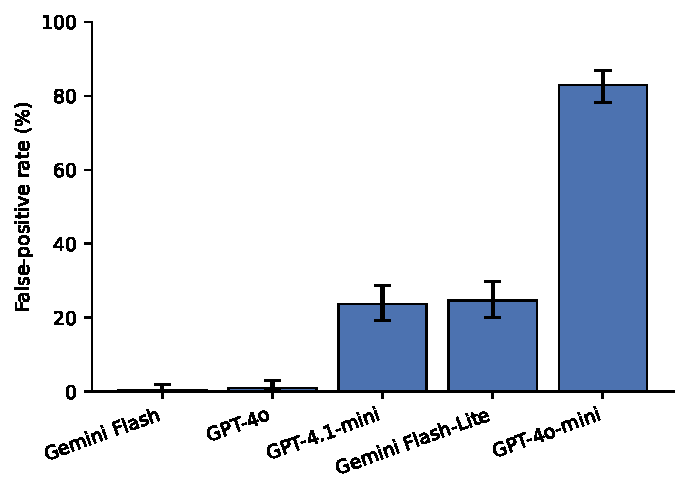
\includegraphics[width=0.72\textwidth]{fig1_fp_by_model.pdf}
\caption{\textbf{False-positive rate of five foundation models on identical legitimate transactions.} Bars show the percentage of 300 legitimate cases each model flagged as suspicious; error bars are 95\% Wilson score confidence intervals. Rates span 0.3--83.0\% (Cochran's $Q=131.6$, degrees of freedom $=4$, $P\approx2\times10^{-27}$).}
\label{fig:fp}
\end{figure}

\begin{figure}[t]
\centering

\includegraphics[width=0.62\textwidth]{fig2_operating_points.pdf}
\caption{\textbf{Each model occupies a different operating point.} Sensitivity (percentage of 300 suspicious cases caught) versus false-positive rate (percentage of 300 legitimate cases flagged) for the five foundation models (circles) and the two non-LLM baselines (triangles: rules heuristic; supervised classifier). Within a provider, the more capable model is not consistently the more conservative.}
\label{fig:ops}
\end{figure}

\begin{figure}[t]
\centering
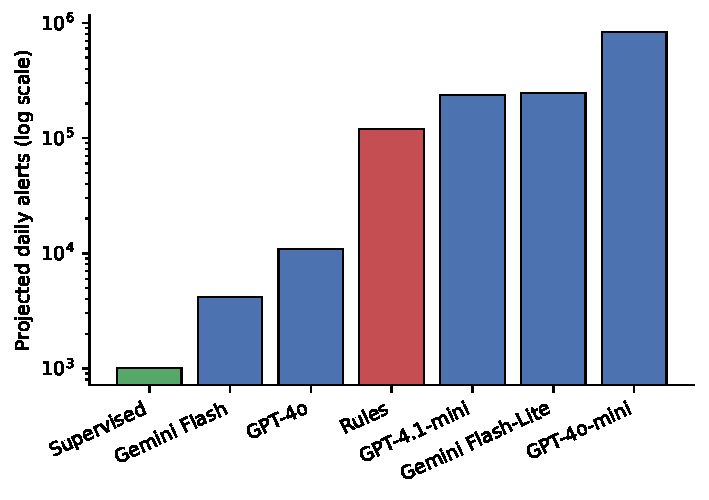
\includegraphics[width=0.72\textwidth]{fig3_alert_volume.pdf}
\caption{\textbf{Projected daily alert workload at realistic prevalence.} Expected daily alerts for each screener at a suspicious prevalence of 0.1\% over 1,000,000 transactions per day (logarithmic axis). Model choice changes the queue from about 4,200 to about 830,000 alerts on identical activity.}
\label{fig:vol}
\end{figure}

\begin{figure}[t]
\centering

\includegraphics[width=0.75\textwidth]{fig4_typology_miss.pdf}
\caption{\textbf{A shared blind spot for trade-based laundering.} Miss rate by laundering typology, pooled across the five models; error bars are 95\% Wilson score confidence intervals. Trade-based laundering and cash-intensive fronts are missed substantially more often than structural typologies.}
\label{fig:typ}
\end{figure}

\begin{figure}[t]
\centering

\includegraphics[width=0.66\textwidth]{fig5_typology_model_heatmap.pdf}
\caption{\textbf{Miss rate by laundering typology and model.} Percentage of suspicious cases of each typology (rows) missed by each model (columns); darker cells indicate more misses. The cautious models (Gemini Flash, GPT-4o) concentrate their misses in trade-based laundering and cash-intensive fronts, while the alert-flooding GPT-4o-mini misses almost nothing---the per-typology signature of the operating-point trade-off in Fig.~\ref{fig:ops}.}
\label{fig:heat}
\end{figure}

\begin{table}[t]
\caption{\textbf{Per-model operating point on the identical 600-case battery.} Values are percentages with 95\% Wilson score confidence intervals; $n=300$ legitimate and 300 suspicious cases.}\label{tab:ops}
\begin{tabular}{@{}llll@{}}
\toprule
Model & Provider & False-positive rate & Miss rate \\
\midrule
Gemini Flash      & Google & 0.3 [0.1--1.9]   & 12.0 [8.8--16.2] \\
GPT-4o            & OpenAI & 1.0 [0.3--2.9]   & 3.3 [1.8--6.0] \\
GPT-4.1-mini      & OpenAI & 23.7 [19.2--28.8]& 3.7 [2.1--6.4] \\
Gemini Flash-Lite & Google & 24.7 [20.1--29.8]& 0.7 [0.2--2.4] \\
GPT-4o-mini       & OpenAI & 83.0 [78.3--86.8]& 0.0 [0.0--1.3] \\
\botrule
\end{tabular}
\end{table}

\begin{table}[t]
\caption{\textbf{Projected daily operational impact at 0.1\% prevalence (1,000,000 transactions/day).} Projected daily-alert counts carry a 95\% interval obtained by propagating the false-positive-rate Wilson interval through the projection; counts are rounded to three significant figures. Rules and supervised baselines are shown for reference; the supervised baseline is an optimistic ceiling on synthetic structure.}\label{tab:vol}
\begin{tabular}{@{}lrlr@{}}
\toprule
Screener & FP rate (\%) & Projected daily alerts (95\% CI) & Precision (\%) \\
\midrule
Supervised (ceiling) & 0.0  & $\sim$1{,}000                    & 100 \\
Gemini Flash         & 0.3  & 4{,}200 (1{,}500--19{,}500)      & 20.9 \\
GPT-4o               & 1.0  & 11{,}000 (4{,}400--29{,}900)     & 8.8 \\
Rules baseline       & 12.0 & 121{,}000 (88{,}700--162{,}000)  & 0.7 \\
GPT-4.1-mini         & 23.7 & 237{,}000 (193{,}000--289{,}000) & 0.4 \\
Gemini Flash-Lite    & 24.7 & 247{,}000 (202{,}000--299{,}000) & 0.4 \\
GPT-4o-mini          & 83.0 & 830{,}000 (784{,}000--868{,}000) & 0.1 \\
\botrule
\end{tabular}
\end{table}

\begin{table}[t]
\caption{\textbf{Pairwise comparison of false-positive rates.} McNemar's exact (binomial) test on the 300 legitimate cases (same cases for all models); $b$ and $c$ are the discordant counts. $P$-values are two-tailed and Bonferroni-corrected across the ten model pairs. The two within-tier pairs (top) are indistinguishable; every between-tier pair is separated at $P<10^{-18}$.}\label{tab:mcnemar}
\begin{tabular}{@{}lrrl@{}}
\toprule
Model pair & $b$ & $c$ & $P$ (Bonferroni) \\
\midrule
Gemini Flash vs GPT-4o                & 1 & 3   & 1.0 \\
GPT-4.1-mini vs Gemini Flash-Lite     & 42 & 45 & 1.0 \\
Gemini Flash vs GPT-4.1-mini          & 1 & 71  & $3.1\times10^{-19}$ \\
Gemini Flash vs Gemini Flash-Lite     & 1 & 74  & $4.0\times10^{-20}$ \\
GPT-4o vs GPT-4.1-mini                 & 0 & 68  & $6.8\times10^{-20}$ \\
GPT-4o vs Gemini Flash-Lite            & 0 & 71  & $8.5\times10^{-21}$ \\
GPT-4.1-mini vs GPT-4o-mini            & 1 & 179 & $2.4\times10^{-51}$ \\
Gemini Flash-Lite vs GPT-4o-mini       & 8 & 183 & $2.5\times10^{-43}$ \\
Gemini Flash vs GPT-4o-mini            & 0 & 248 & $4.4\times10^{-74}$ \\
GPT-4o vs GPT-4o-mini                  & 0 & 246 & $1.8\times10^{-73}$ \\
\botrule
\end{tabular}
\end{table}

\backmatter

\bmhead{Data availability}
The synthetic battery generator, the frozen 12{,}000-call dataset, the analysis code, the frozen preregistration, and a one-command reproducible capsule (which regenerates and hash-verifies the battery, recomputes every reported statistic, and confirms byte-identical outputs across runs) are openly available in a public repository and Code Ocean capsule [persistent DOI to be inserted on acceptance]. All numbers reported here, with their confidence intervals and the configuration hash that produced them, are included as a machine-readable file in that repository.

\bmhead{Acknowledgements}
Analyses used open-source software (Python, NumPy, scikit-learn, SciPy, Matplotlib); the author thanks their maintainers.

\section*{Declarations}

\textbf{Competing interests.} The authors declare no competing interests.

\textbf{Author contributions.} S.C. conceived the study, designed and preregistered the analysis, implemented the data-collection and analysis software, performed the experiments and analysis, and produced the figures. R.C. contributed to the study design, the interpretation of results, and the critical revision of the manuscript. Both authors wrote, reviewed and approved the final manuscript.

\textbf{ORCID.} S.C. 0009-0007-2779-3492; R.C. 0009-0007-2807-3948.

\textbf{Ethics approval.} Not applicable (synthetic data only; no human participants, human tissue or animals).

\bibliography{sn-bibliography}

\end{document}
